% Template for PLoS
% Version 1.0 January 2009
%
% To compile to pdf, run:
% latex plos.template
% bibtex plos.template
% latex plos.template
% latex plos.template
% dvipdf plos.template

\documentclass[10pt]{article}

% amsmath package, useful for mathematical formulas
\usepackage{amsmath}
% amssymb package, useful for mathematical symbols
\usepackage{amssymb}

% graphicx package, useful for including eps and pdf graphics
% include graphics with the command \includegraphics
\usepackage{graphicx}

% cite package, to clean up citations in the main text. Do not remove.
\usepackage{cite}

\usepackage{color} 

% Use doublespacing - comment out for single spacing
%\usepackage{setspace} 
%\doublespacing


% Text layout
\topmargin 0.0cm
\oddsidemargin 0.5cm
\evensidemargin 0.5cm
\textwidth 16cm 
\textheight 21cm

% Bold the 'Figure #' in the caption and separate it with a period
% Captions will be left justified
\usepackage[labelfont=bf,labelsep=period,justification=raggedright]{caption}

% Use the PLoS provided bibtex style
\bibliographystyle{plos2009}

% Remove brackets from numbering in List of References
\makeatletter
\renewcommand{\@biblabel}[1]{\quad#1.}
\makeatother


% Leave date blank
\date{}

\pagestyle{myheadings}
%% ** EDIT HERE **


%% ** EDIT HERE **
%% PLEASE INCLUDE ALL MACROS BELOW

%% END MACROS SECTION

\begin{document}

% Title must be 150 characters or less
\begin{flushleft}
{\Large
\textbf{ClinicalCodes: An online clinical codes repository to improve the validity and reproducibility of research using electronic medical records}
}
% Insert Author names, affiliations and corresponding author email.
\\
David A Springate$^{1,2,\ast}$, 
Evangelos Kontopantelis$^{1,3}$,
Darren M Ashcroft$^{4}$,
Ivan Olier$^{5}$,
Rosa Parisi$^{4}$,
Edmore Chamapiwa$^{1}$,
David Reeves$^{1,2}$
\\
\bf{1} Centre for Primary Care, Institute for Population health, University of Manchester, Manchester, UK
\\
\bf{2} Centre for Biostatistics, Institute for Population health, University of Manchester, Manchester, UK
\\
\bf{3} Centre for Health Informatics, Institute for Population health, University of Manchester, Manchester, UK
\\
\bf{4} Centre for Pharmacoepidemiology and Drug Safety Research, Manchester Pharmacy School, University of Manchester, Manchester, UK
\\
\bf{5} Manchester Institute for Biotechnology, University of Manchester, Manchester, UK
\\
$\ast$ E-mail: Corresponding david.springate@manchester.ac.uk
\end{flushleft}

% Please keep the abstract between 250 and 300 words
\section*{Abstract}

Lists of clinical codes are the foundation for research undertaken using electronic medical records and without access to them, reviewers are unable to determine the validity of research, full replication is impossible and researchers are unable to make effective comparisons between studies and are subject to much duplication of effort in building new code lists.  Despite this, publication of clinical codes is rarely if ever a requirement for obtaining grants, validating protocols or publishing research.  We have built a centralised online repository where researchers using electronic medical records can upload and download lists of clinical codes to help address these problems.  The repository will enable clinical researchers to better validate electronic medical records studies, build on previous code lists and compare disease definitions across studies.  It will also assist health informaticians in replicating database studies, tracking changes in disease definitions or clinical coding practice through time and sharing clinical code information across platforms and data sources as research objects. 

\section*{Introduction}

Over the last 20 years, increasing numbers of general practitioners have used computers to store patients medical records for various administrative functions \cite{Purves1996}. Hospitals are also beginning to store their records electronically, though electronic records are far less prevalent than in primary care \cite{Ashish2009}. These electronic medical records (EMRs) offer great potential for research, enabling the rapid identification of patients for inclusion in intervention and observational studies. As their use becomes more widespread, it is becoming increasingly important to have better means for ensuring and evaluating the validity of studies based on EMRs. EMRs are being used by researchers to address important questions in healthcare that would be difficult or impossible to address using randomised controlled trials, because of the costs involved, the low prevalence of conditions or because a condition may occur in a subgroup such as children or pregnant women. In UK primary care in particular, the annual number of research outputs based on the three main UK primary care databases (The Clinical Practice Research Datalink (CPRD, formerly the General Practice Research Database, GPRD), The Health Improvement Network (THIN) and QResearch) appears to be increasing at an exponential rate (figure \ref{figure1_articles_per_year}). 


Much research has been done into establishing the internal and external validity of EMR studies \cite{Herrett2010}, particularly from the point of view of data quality, data completeness and confounding.  The validity of morbidity registers has also received much attention, through comparison with other sources \cite{Jordan2004}. There has also been some work replicating studies from one EMR database in another to assess their external validity \cite{Hippisley-Cox2008, Vinogradova2013, Reeves2014}.  Notwithstanding all of these efforts to establish general validity, most EMR studies adopt bespoke definitions of clinical entities (such as disease conditions, treatments and diagnostic tests) that are seldom questioned or challenged.  These clinical entities are defined through lists of `clinical codes' and the process of preparing these code lists is rarely straightforward and often lacks rigor \cite{Dave2009}.  Despite calls for greater transparency and sharing of code lists and also for greater use of sensitivity analyses using different sets of codes \cite{Gulliford2009, Bhattarai2012}, code lists are still seldom reported in published papers \cite{Herrett2010}.  There is also currently no obligation from funding bodies, journals or regulators for researchers to publish their code lists.  Furthermore, there is no centralised repository to hold lists of clinical codes. Consequently, it is impossible to assess the validity of the vast majority of code lists used in EMR research. 

There is also a gradual movement towards greater transparency and openness in academic research \cite{Bechhofer2013, Stodden2013, Pampel2013}, sometimes driven by learned societies \cite{RoyalSoc2012}, particularly in disciplines where there is high computational load. Furthermore, there is growing pressure from governmental organisations to share and open access to publicly funded research data \cite{EuropeanCommission2012, OfficeSciTech2013}.

To facilitate the transition towards full transparency, we developed www.ClinicalCodes.org, a web repository for EMR researchers to freely upload and download clinical code lists.  Below we give an overview of the role and use of clinical codes in EMR research and provide details on the features of the ClinicalCodes repository.


\section*{The role of clinical codes in EMR databases and research}


Clinical entities in EMR databases are entered by medical professionals as clinical codes.  In UK primary care, Read codes (named after Dr. James Read) are the most commonly used, while the ICD-9/10 system (adopted by the World Health Organisation)  is more popular in UK hospital settings and primary care in North America and mainland Europe.  These codes form a hierarchical classification system for reporting and research purposes and are the essential `building blocks' used to define symptoms, signs and diagnoses, referrals to hospitals and clinics, immunisations, prescribed medications and diagnostic test results.

The process of drawing up code lists to identify clinical entities of interest (e.g patients with a given clinical condition, patients on particular medications, patients with certain diagnostic test, smoking status etc.) is a critical step in setting up EMR studies and multiple code lists will often be required within one study to define multiple conditions, covariates, confounders and outcomes.  This is often a complicated and time-consuming process that involves defining the clinical entity of interest and iteratively searching for codes in lookup tables, running searches for codes in different sections of the database, collating the results and classifying them (generally by clinically trained investigators) \cite{Dave2009, Nicholson2013}.  The built in flexibility and redundancy of clinical coding systems allows practitioners to use a variety of codes to describe a given condition and minimises their time spent searching for codes, but it presents a challenge to researchers using these codes to effectively define a clinical entity. A patient may receive one of several possible diagnostic codes as well as, or instead of, one or more codes describing symptoms or investigations. This flexibility in the coding structure facilitates the clinical use of these codes and minimises the time spent searching for codes by practitioners. However, the multitude of codes for a given condition presents a challenge when data need to be aggregated. For example, the definition of a particular disease condition could include a combination of codes representing diagnoses, symptoms, prescribed drugs and diagnostic tests in order to accurately identify all patients with a certain complicated condition.  On the other hand, some entities can be identified with a very simple code list, or even a single clinical code \cite{Kotz2011}.


In any particular application, the set of codes used to define the relevant clinical entities will vary according to the particular question being asked, partly reflecting the sensitivity (or specificity) required by the definition. In some instances it is more important to be all-inclusive and use a broad definition so as not to miss any potential cases; but at other times a narrower definition may be required to focus on cases where diagnosis is more certain.  Precisely how a code list is specified can have a major impact on the results of a study \cite{Nicholson2011}. For example, a sevenfold variation in estimates of incidence of rheumatoid arthritis can be largely explained by differences in code-lists between different studies \cite{Garcia2009, Watson2003}.  To account for such variation some studies have used different subsets of code-lists in sensitivity analyses \cite{Doran2011, Herrett2010}.  Furthermore, and in particular for uncommon diseases, small errors in code selection can result in large numbers of misclassified patients, leading to biased results and classification errors affecting conclusions in unpredictable ways \cite{Manuel2010}. Clinical definitions may also change over time, resulting in a need to revise the corresponding code list \cite{Gulliford2009}, a good example being a change in the UK Quality and Outcomes Framework (QOF) Business Rules in 2006. When QOF was first introduced, people with diabetes were identified on the basis of any diabetes code, including non-specific diabetic type codes.  From April 2006, the case definition for diabetes was restricted to include only those codes that specified type I or type II diabetes \cite{Hippisley-Cox2006}.  In practice this meant that about 170 previously used Read codes were no longer being used to identify the condition. Finally, different researchers may have different interpretations of the relevance of particular codes.

\section*{Reporting of codes in the current literature}

A large component of total EMR research is made up by primary care database (PCD) studies and UK PCDs are among the most researched in the world.  Figure \ref{figure1_articles_per_year} shows that research outputs with UK PCDs appears to be increasing at an exponential rate, while figure \ref{figure2_PCD_map} shows that research using UK PCDs is being conducted in universities, pharmaceutical companies and research hospitals around the world, and is not just limited to the UK.  As one of the largest and most important resources for EMR-based research, it seems reasonable to expect reporting of code lists in UK PCD-based studies to be at least as comprehensive as in other EMR studies.  To evaluate levels of transparency in the reporting of clinical code lists, we took a representative sample of UK PCD studies and assessed each study on its extent of reporting of the clinical codes used.

We took a sample of 450 papers from the original 1359 identified from a PubMed search.  Of these, 392 (87\%) had both  the full text accessible to the University of Manchester library and were examples of primary PCD research.  Only 35 (9\% of 392) studies published the entire set of clinical codes needed to reproduce the study (usually in an online appendix), while only an additional 47 (12\%) stated explicitly that the clinical codes are available upon request \ref{tab:table1_percentages}.


\section*{The need for transparency in clinical code usage}


We identify four main consequences of lack of transparency of clinical code lists.  First, if code lists are not made available or not published alongside the primary research using them, they represent an important part of a study methodology that is not subject to scrutiny or peer review. In the extreme case, there is no way of assessing the validity of the diagnosis definition used in a study and clinical decisions could be based on invalid results derived from an incorrect patient base.  This could happen despite rigorous downstream statistical analysis.  Second, the effective replication of EMR studies is dependent on the availability of the clinical codes from the original study.  If all of the codes are not available, it is impossible to tell if differences found in study replications are due to artefactual differences in code lists or if they are genuine.  Third, if code-lists are unknown, comparisons between studies addressing the same clinical question are potentially invalidated.  Condition definitions change over time and GP coding practice may also change with respect to regulations and incentives \cite{Hippisley-Cox2006}. Also, different studies may use different types of codes for a condition; some studies, for example, include medication and monitoring codes as part of their definition of a patient with diabetes (e.g. \cite{Mulnier2006}) while others do not (e.g. \cite{Kontopantelis2014}).  Not having access to code-lists means that it is difficult to know whether fair comparisons are being made between studies. Fourth, building code lists is a time consuming process; having access to historical code lists  would mean that new lists could be built incrementally and iteratively, saving much `reinvention of the wheel' while increasing consistency, and potentially accuracy, of definitions across studies.



\section*{The ClinicalCodes online repository}

The main ClinicalCodes database consists of a set of `Articles', for each of which a code list, or a collection of code lists, has been uploaded onto the ClinicalCodes.org site. These articles may be, for example, peer-reviewed papers published in medical journals, or other important sources of code lists such as the QOF Business Rule sets (Figure 3). Alongside each article is included  metadata such as an abstract, citation details, a contact name where possible, and in the case of journal papers, a link to the full text article and DOI. For each article, the associated code lists are detailed and within these the individual clinical codes making up the list.  All individual clinical codes are assigned a code name, coding system (Read, OXMIS, SNOMED, CPRD\_product\_code, BNF\_code, OXMIS, ICD-9, ICD-10), description and entity type (diagnostic, drug, test, clinical\_sign, administrative, demographic, observation, immunisation).  Users are able to upload supplementary fields for individual codes or add comments at the code list or article level.  Code lists can be downloaded by any user but an account must be created to upload article metadata or code lists or to leave comments. Code lists can be downloaded individually as csv files. If a code lists from a previous article has been used verbatim in a new study, the ClinicalCodes entry for the new study can link to the previous code list.  This reduces workload in uploading lists that are unchanged from previous studies while retaining information on the origin of code lists.  At the time of publication, the complete code lists used for three papers from our group \cite{Doran2011, Kontopantelis2014, Reeves2014} as well as codes from the UK Quality and Outcomes Framework Business rules versions 5 and 24 - a total of 15193 clinical codes across 105 code lists covering medical conditions, lifestyle variables (such as smoking status) physical observations (such as BMI) and testing (for example for retinal screening and blood sugar levels).

We have endeavored to make the upload and download processes as straightforward as possible. In particular, download of individual code lists is a one-click operation requiring no log in or provision of user information.  The comments feature, which is available for articles and code lists, enables the study authors to add extra methodological information and also allows other researchers to raise questions and make observations on the code lists which could further assist the development of future code lists.

We have also developed an open-source R package \cite{Springate2014} to automate the downloading and importing of clinical code lists from ClinicalCodes.

%%%  RECYCLING CODELISTS FEATURE IS STILL TO BE IMPLEMENTED!   %%%    

\subsection*{Clinical Codes as research objects}

%%%% ro stuff not yet implemented in ClinicalCodes.. %%%%

Research objects are annotated aggregations of data often associated with a scientific publication that facilitate reuse and reproducibility of scientific research \cite{Bechhofer2010}. Following this model, metadata and links to code lists for articles are available as research objects that can be shared across platforms in machine readable form.  In practice, this means that a JSON manifest file is available for each article containing: Article metadata (title, author, abstract, reference, link, doi), article level comments, code list level comments and links to the individual code list files. These research object files are available directly by adding a `/ro' to the URI for an article (e.g. www.clinicalcodes.org/medcodes/article/5/ro).  The research object format is designed to be available without getting in the way of the main method of download that will be required by most users.  The rClinicalCodes R package \cite{Springate2014} enables the automated download of code lists and metadata via the research object file. An example JSON manifest file is shown in the online appendix.

\section*{Conclusions}

% Biosharing.org
% re3data.org
% force11.org

Large electronic medical datasets, including medical records datasets are already playing an important role in clinical research and this role is set to grow in the era of big data in healthcare \cite{Wang2013}. The successful exploitation of big data in healthcare will depend on the ability of researchers to access and validate that data and then combine it with other sources \cite{Murdoch2013}.  We have developed a repository for clinical codes that will be of great use to two groups of researchers.  First, clinical researchers using primary care and other medical databases will be able to more effectively validate their research, build upon previous code lists and match appropriate disease definitions through time. Second, health informaticians will more easily be able to produce study replications (e.g. replications across databases such as \cite{Reeves2014}), share clinical code data as research objects across platforms and data sources and use the ClinicalCodes database as a research resource in its own right (e.g. to track changes in disease definitions and clinical coding practice through time).

Researchers using the ClinicalCodes repository can benefit from faster and more consistent development of new code lists, improvements in research quality associated with better scrutiny of lists of clinical codes, greater exposure and potential for studies with uploaded codes to have greater visibility and impact and also from discovering other researchers working in the same area.

Despite these motivations, the success of this project will depend on its widespread adoption by the electronic medical records research community. Although ClinicalCodes solves the problem of having a centralised repository for holding codes, the problem remains that there are few, if any, requirements for researchers to make clinical code lists accessible. We believe that adoption and support of a centralised clinical codes repository by regulators, funding bodies and publishers of electronic medical records research will be of great benefit to the electronic medical records research community.

\subsection*{Availability and Requirements}

%%% Not yet indexed....  %%%%

ClinicalCodes is freely accessable at http://www.clinicalcodes.org.

\section*{Materials and Methods}

\subsection*{Article Classification}

To get an estimate of the extent of the problem of lack of transparency in clinical code-lists in EMR studies, we collected articles conducting primary research using the three major UK-wide Primary care databases (PCDs) (The Clinical Practice Research Datalink, formerly the General Practice Research Database; The Health Improvement Network; QResearch).  A Search was made on Pubmed for articles with the following terms: ``CPRD'', ``Clinical Practice Research Datalink'', ``GPRD'', ``General Practice Research Database'', ``The Health improvement Network'', ``QResearch'' up until September 2013, returning 1359 articles.  A random sample of 450 articles was taken for further analysis.  From this sample, all articles were identified that were both primary EMR research and had their full text accessable via the University of Manchester library (392 articles). We then scored each paper as belonging or not to each of the following categories:

\begin{enumerate}
    \item Any clinical codes listed in the methods section
    \item At least one full code list provided in the paper or in an appendix
    \item All code lists provided to enable replication of the study
    \item States that ``Code lists are available on request'' 
\end{enumerate}

Analyses were performed using R v2.15.2 \cite{R2012}. Article counts over time and geo-coded article affiliations (Via the Google Geocoder API) were aggregated using the R package rpubmed (https://github.com\slash rOpenHealth/rpubmed).

\subsection*{Database Architecture and Web Interface}

The repository data is stored in a relational database called PostgreSQL (http://www.postgresql.org). Server-side web programming was done in Python v2.7.5 (http://www.python.org) using the Django v1.5 web framework (https://www.djangoproject.com). The client side scripting was done in JavaScript and HTML5 and used Twitter Bootstrap v3 (http://getbootstrap.com) as a front-end framework.  The dynamic parts of the site were served using Gunicorn v18.0 (http://gunicorn.org) and static parts with Nginx v1.0.15 (http://nginx.org). Cacheing and sessions are handled by a Redis v2.4.10 NoSQL database (http://redis.io). The repository is hosted on a 64 bit Red Hat Enterprise Linux server release 6.4 virtual machine at the University of Manchester. 


% Do NOT remove this, even if you are not including acknowledgments
\section*{Acknowledgments}
We are thankful to Matt Ford for extensive technical support. Thanks to the Research team at CPRD for fruitful discussions in the development stage.

\subsection*{Funding statement}
This work is funded by the National Institute for Health Research (NIHR) School for Primary Care Research (SPCR).

\subsection*{Disclaimer}
This article/paper/report presents independent research funded by the National Institute for Health Research (NIHR).  The views expressed are those of the author(s) and not necessarily those of the NHS, the NIHR or the Department of Health.

\section*{Author Contributions}

Conceived, designed and built the website and software: DAS. Data collection: DAS, DR, EK, IO, RP, DA, EC.  Data Analysis: DAS. Wrote the manuscript DAS. Edited the manuscript DAS, DR, EK, IO, RP, DA, EC.

%\section*{References}
% The bibtex filename
\bibliography{clinicalcodes}

\section*{Tables}

\begin{table}[!ht]
  \caption{
    \bf{Percentages of a random sample of UK primary care database studies with details of code lists}}
  \begin{tabular}{|c|c|c|}
    \hline
                 & Number of articles & Percentage \\
    \hline
    All UK PCD articles        & 1359 & ---  \\
    In random sample           & 450  & ---  \\
    Full-text available        & 417  & ---  \\
    Primary PCD research       & 392  & 100  \\
    Any code in methods        & 104  & 26.5 \\
    Any code list in study     & 74   & 18.9 \\
    All relevant code-lists    & 34   & 8.7  \\
    Any codes in paper         & 117  & 29.8 \\
    Codes available on request & 48   & 12.2 \\
    Any codes or available     & 138  & 35.2 \\
    \hline
  \end{tabular}
  \begin{flushleft}Percentages are relative to the number of primary PCD research studies 
  \end{flushleft}
  \label{tab:table1_percentages}
\end{table}


\section*{Figure Legends}

\begin{figure}[!ht]
\begin{center}
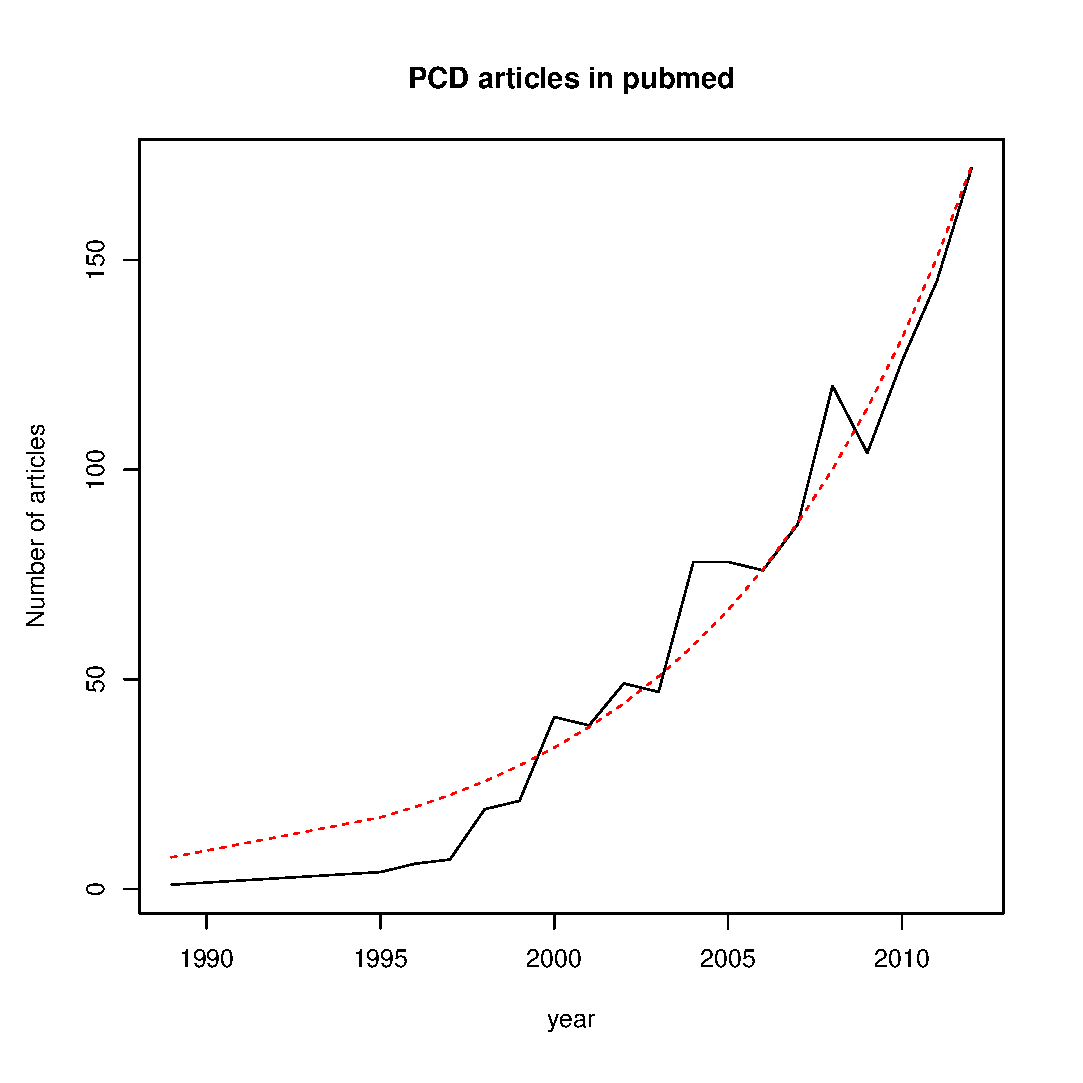
\includegraphics[width=4in]{figure/articles_per_year.eps}
\end{center}
\caption{
    {\bf Number of UK Primary Care Database publications.}
}
\label{figure1_articles_per_year}
\end{figure}

\begin{figure}[!ht]
\begin{center}
  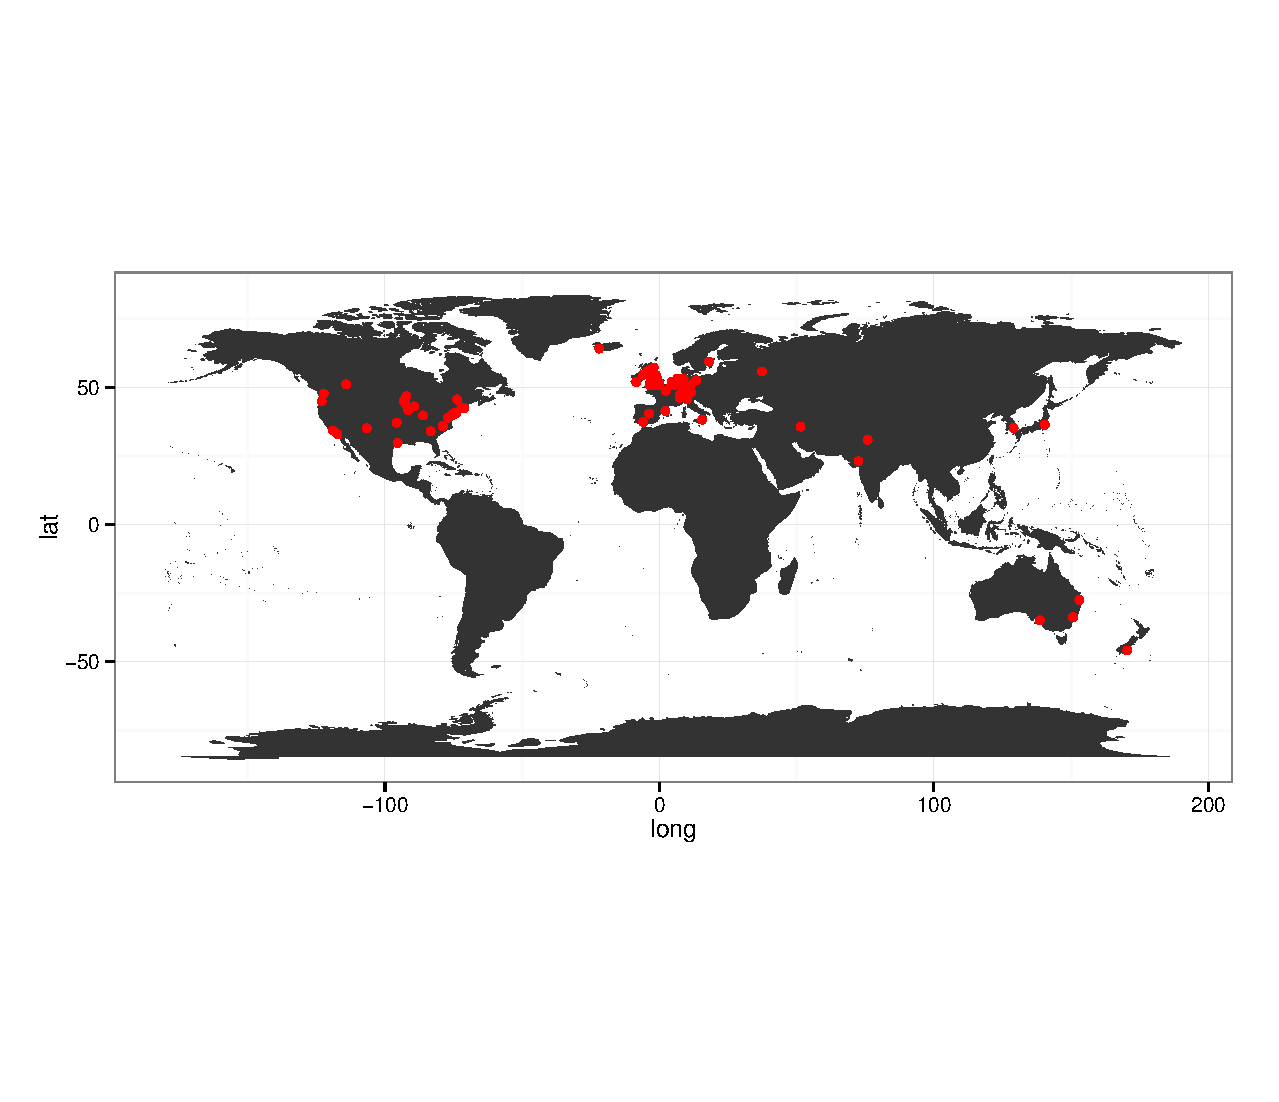
\includegraphics[width=4in]{figure/PCD_world.eps}
\end{center}
\caption{
    {\bf Locations of primary affiliated departments.}
}
\label{figure2_PCD_map}
\end{figure}

\begin{figure}[!ht]
\begin{center}
  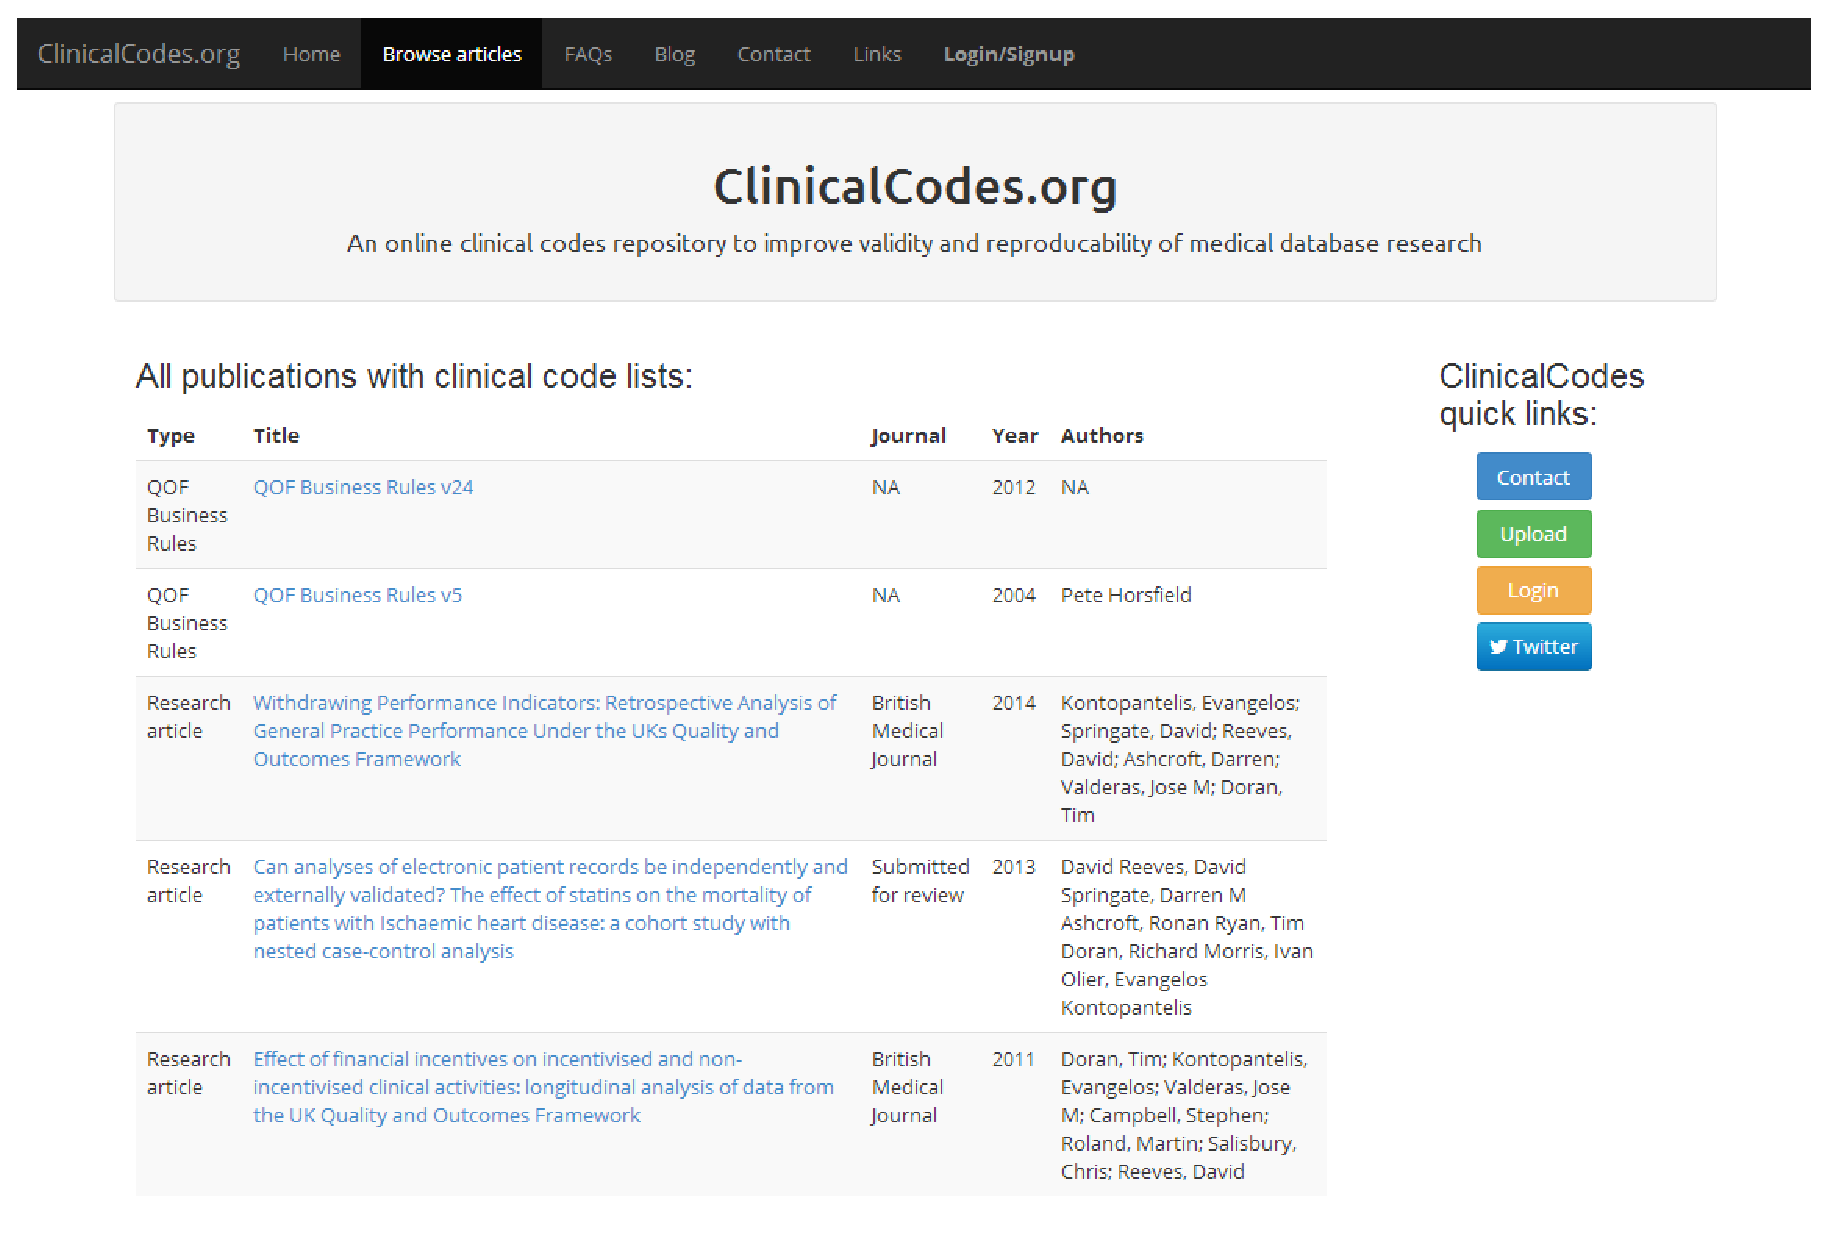
\includegraphics[width=6in]{figure/clinicalcodes_screenshot.eps}
\end{center}
\caption{
    {\bf Screenshot of the ClinicalCodes website showing articles with uploaded code lists.}
}
\label{figure2_PCD_map}
\end{figure}


\end{document}

